
%(BEGIN_QUESTION)
% Copyright 2007, Tony R. Kuphaldt, released under the Creative Commons Attribution License (v 1.0)
% This means you may do almost anything with this work of mine, so long as you give me proper credit

Examine this network diagram of an industrial data acquisition system, comprised of different technologies for acquiring the data, but ultimately communicating to computer display stations located somewhere on the Internet (world wide web):

$$\includegraphics[width=15.5cm]{i02236x01.eps}$$

Identify some of the different OSI layer 1 (physical) network standards you see in this system, as well as OSI layer 2 (data link) addressing schemes.  Then, explain how all this data, in all its different forms, gets shuttled over the same ISDN cable to the Internet using TCP/IP packets.

\vskip 20pt \vbox{\hrule \hbox{\strut \vrule{} {\bf Suggestions for Socratic discussion} \vrule} \hrule}

\begin{itemize}
\item{} Identify where the diagnostic utlility {\tt ping} could be used to test nodes in this heterogeneous network.
\item{} Identify where the diagnostic utlility {\tt ping} could {\it not} be used to test nodes in this heterogeneous network.
\end{itemize}

\underbar{file i02236}
%(END_QUESTION)





%(BEGIN_ANSWER)

Some of the different OSI layer 1 formats seen here:

\begin{itemize}
\item{} EIA/TIA-232
\item{} EIA/TIA-485
\item{} Bell 202 (HART FSK signals)
\item{} DeviceNet
\item{} Ethernet 10BASE-T (IEEE 802.3)
\item{} IEEE 802.11g (wireless)
\end{itemize}

\vskip 10pt

Some of the OSI layer 2 addressing schemes seen here:

\begin{itemize}
\item{} HART field device addresses
\item{} MAC addresses for each personal computer
\end{itemize}

\vskip 10pt

The personal computers are responsible for ``wrapping'' the disparate data streams into TCP/IP packets, which are then forwarded to the router over Ethernet, then transmitted over ISDN.  Once in packetized form, they become portable over any network standard, requiring only a computer with an ``understanding'' of TCP/IP protocol to reassemble and ``unwrap'' at the receiving end(s).

%(END_ANSWER)





%(BEGIN_NOTES)

One thing I have left out of this question (and answer!) is the software that can make sense of all these data streams, both on the server (DAQ) side and the client (display) side.  OPC would be great, but that's a topic I prefer to deal with later . . .

\vskip 10pt

Remember that {\tt ping} is based on IP (Internet Protocol) and as such only works with devices having an IP address.










\filbreak \vskip 20pt \vbox{\hrule \hbox{\strut \vrule{} {\bf Virtual Troubleshooting} \vrule} \hrule}

\noindent
{\bf Predicting the effect of a given fault:} present each of the following faults to the students, one at a time, having them comment on all the effects each fault would produce.

\begin{itemize}
\item{} Ethernet cable to left PC fails
\item{} Ethernet cable to middle PC fails
\item{} Ethernet cable to right PC fails
\item{} 232/485 converter fails
\item{} ISDN router fails 
\item{} Terminator removed from DeviceNet network
\end{itemize}


\vskip 10pt


\noindent
{\bf Identifying possible/impossible faults:} present symptoms to the students and then have them determine whether or not a series of suggested faults could account for all the symptoms, explaining {\it why} or {\it why not} for each proposed fault:

\begin{itemize}
\item{} Symptom: {\it PLC cannot read data from HART transmitter \#3}
\item{} ISDN network cable failed -- {\bf No}
\item{} HART modem failed -- {\bf Yes}
\item{} ISDN router failed -- {\bf Yes}
\item{} WAP failed -- {\bf No}
\item{} DeviceNet terminator missing -- {\bf No}
\item{} RS-232/485 converter failed -- {\bf Yes}
\item{} Right PC jabbering on Ethernet -- {\bf Yes}
\vskip 10pt
\item{} Symptom: {\it PLC reads false breaker status from protective relay \#7 (shows breaker to be closed when it is in fact it has been tripped open by that relay)}
\item{} CT failed shorted on relay \#7 -- {\bf No}
\item{} HART modem failed -- {\bf No}
\item{} DeviceNet terminator missing -- {\bf Yes}
\item{} ISDN router failed -- {\bf Yes}
\item{} ISDN network cable failed -- {\bf No}
\item{} RS-232/485 converter failed -- {\bf Yes}
\item{} WAP jabbering on Ethernet -- {\bf Yes}
\end{itemize}


\vskip 10pt


\noindent
{\bf Determining the utility of given diagnostic tests:} present symptoms to the students and then propose the following diagnostic tests one by one.  Students rate the value of each test, determining whether or not it would give useful information (i.e. tell us something we don't already know).  Students determine what different results for each test would indicate about the fault, if anything:

\begin{itemize}
\item{} Symptom: {\it HART transmitter \#4 data unavailable on world-wide web}
\item{} Ping 196.244.10.2 from one of the computer display stations -- {\bf Yes}
\item{} Ping 196.244.10.4 from one of the computer display stations -- {\bf Yes}
\item{} Inspect Rx/Tx LEDs on HART modem -- {\bf Yes}
\item{} Check for live data from HART transmitter \#2 on the world-wide web -- {\bf Yes}
\item{} Inspect LEDs on ISDN router port for middle PC cable -- {\bf Yes}
\end{itemize}


\vskip 10pt


\noindent
{\bf Diagnosing a fault based on given symptoms:} imagine the ??? fails ??? in this system (don't reveal the fault to students!).  Present the operator's observation(s) to the students, have them consider possible faults and diagnostic strategies, and then tell them the results of tests they propose based on the following symptoms, until they have properly identified the nature and location of the fault:

\begin{itemize}
\item{} {\it }
\item{} 
\item{} 
\end{itemize}
%INDEX% Networking, protocol: TCP/IP used to ``glue'' heterogeneous networks together

%(END_NOTES)


